\chapter{Facebook Privacy}
\label{chp:defaultprivacysettings} 

In this chapter we are going to look into what kind of privacy settings that exist on Facebook. We will also look at, and map, how the default privacy settings has evolved over time. In addition to this, we will describe some of the features introduced by Facebook over the years, and how these features have affected the privacy on Facebook. Finally, we will review some of Mark Zuckerberg's  thoughts and comments in regard to Facebook privacy. 


\section{Privacy on Facebook}\label{sec:privacy_on_facebook}

\begin{figure}[b]
\centering
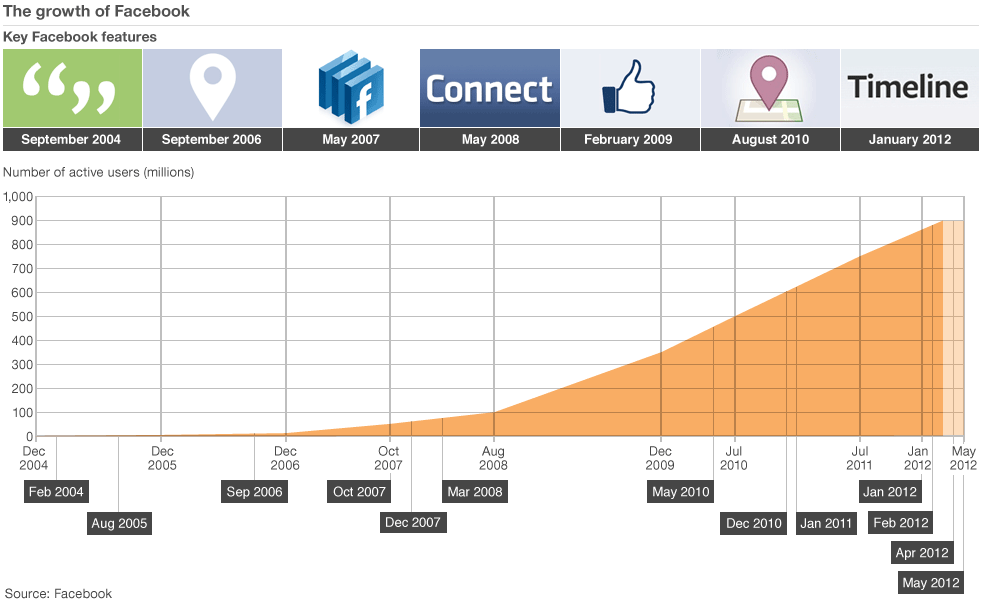
\includegraphics[width=0.8\textwidth]{gowth_of_facebook.png}
\caption[The development of Facebook users and introduction of new features]{\textbf{The development of Facebook users and introduction of new features.} The orange field in the graph shows the increasing number of Facebook users over the years. Key Facebook features are shown over the graph according to when they were introduced \cite{BBCFacebookGrowth}.} 
\label{fig:growth_of_facebook}
\end{figure}

There is no doubt that Facebook has had a remarkable development, both when it comes to number of active users and the development of new features, as shown in \fref{fig:growth_of_facebook}. Along with new users and new features, there has also been made major changes to what kind of privacy settings exists and what kind are needed. 


\subsection{Facebook Settings}
Whenever Facebook make an update to the settings, the users usually get a personal message informing them about the change. Because of the high number of users, this change happens gradually. This means that not everyone will get a notification about the changes made at the same time \cite{settingschangingagain}. Despite the changes over time, the main control of ones privacy lies in the hands of the users. The users have the opportunity to make their profile more secure, than what is default. 

\subsubsection{The settings that exists}
There exists numerous settings one can edit to make their Facebook profile more, or less, secure/private. The main reason why people do not change their settings is probably because they are unaware of the settings' existence. Another problem can be that people are not confident enough in changing them. When they do not know what a setting does, it can be scary to change it. Regardless of this, the settings exists, and it is up to each user how they are configured. 
On the Facebook settings page there is different tabs regarding different kind of settings. The settings available are elaborated in \tref{tab:settings}.

\newpage

\begin{center}
    \begin{longtable}{ | l | p{9cm} |}
    \caption{\label{tab:settings}The settings that exist on Facebook 				\cite{facebooksettings}.} \\
    \hline
    \textbf{Setting tab} & \textbf{Description} \\ 
    \hline
    General & Under this tab the user can edit name, username, email, password, network and language. \\
    \hline
    Security & Under this tab the user can do changes that makes it harder for someone else to hack into the Facebook account. Here the user can enable/disable \textbf{Secure Browsing} (the use of https). It is possible to turn on \textbf{Login Notification}. This means the user will get notified either by email or text message when the account is being accessed from a computer or mobile device that has not been used before. It is possible to enable something called \textbf{Login Approvals}, where a security code is required to access the account from an unknown browser. This code can be given to the user in a text message. The user has the choice to use \textbf{Code Generator} on the Facebook mobile app to reset password or generate login approval security codes. Under the security tab the user can create \textbf{App Passwords}, add \textbf{Trusted Contacts}, view \textbf{Recognized Devices} and \textbf{Active Sessions}. Under active sessions the user can see all sessions active via the user's Facebook account. Here the user can look for unfamiliar devices or locations, and if the user find a session that is unfamiliar, someone else may have been logged onto the account. This session can easily be ended. \\ 
    \hline
    Privacy & Under this tab the user can change the audience for future posts. The user can also choose who can send friend requests, who can look you up using the email address provided and who can look you up using the phone number provided. The last setting concerns whether or not the user want other search engines to link to the user's timeline. This can either be turned On or Off.\\
    \hline
    Timeline and Tagging & Under this tab the user can choose who can post on the timeline, who can see posts you have been tagged in on your timeline and who can see what others post on your timeline. The user can also choose whether or not he/she want to review tags people add to own posts before the tags appear on Facebook, and the user can choose the audience for a post the user has been tagged in, if they are not already in it.\\
	\hline
    Blocking & Under this tab the user can block other users, app invites from specific users, event invites and specific apps. Under this tab the user can also make a \textbf{Restricted List}. These friends will only be able to see the information and posts that are public.\\
    \hline
    Notifications & Under this tab the user can control how to get notifications, and what to get notified about.\\
    \hline
    Mobile & Under this tab the user can add phone number(s), and activate registered phone(s) for text messaging.\\
    \hline
    Followers & Under this tab the user can turn on follow, this makes it possible for other people to follow the user. Followers will only see public posts and will not be added as friends.\\
    \hline
    Apps & Here the user can choose whether or not he/she want to use apps, plugins, games and websites on Facebook and elsewhere. The user also gets a list of the apps installed, and can edit the audience for what is posted via these apps. The people on Facebook who can see a user's information can bring this information with them when they use apps. This is to improve the user experience. Under \textbf{Apps other use} the user can control the categories of information that people can bring with them when they use apps, games and websites. The user can also turn on something called \textbf{Instant personalization}, which let the user see relevant information about friends the moment the user arrive on a select partner website. Finally, under this tab the user can choose the audience for the things posted using old Facebook mobile apps that do not have the in-line audience selector.\\ 
    \hline
    \end{longtable}
\end{center}



\section{Default Settings on Facebook}\label{sec:default_privacy_settings}

Facebook has evolved from being a networking site for students attending Harvard, to becoming a global phenomenon. Facebook's user interface has gone through several changes over the years, which has brought both joy and frustration to the users. When these changes have been made, there has also been made adjustments to the default privacy settings \cite{EvoPriv2}. At the beginning, in 2005, when Facebook first was applied outside of Harvard University, a user's personal information was only accessible to the user's Facebook friends and to people connected to the same network on Facebook \cite{EvoPriv}. This is far from reality today. We will now look into how the default privacy settings on Facebook has evolved over time. 


\subsection{Development of Default Settings}

The main changes to the default privacy settings are emphasized in \tref{tab:dps}. Each year only states the changes made that year. If no changes were made the default settings from the previous year are the valid ones. 

\begin{center}
\begin{longtable}{ | p{1.3cm} | p{10.6cm} |}
\caption{\label{tab:dps}Changes in the default privacy settings on Facebook from 2005 until today \cite{EvoPriv,PrivTimeline}.}\\
    \hline
    \textbf{Year} & \textbf{Default Privacy Settings} \\ 
    \hline
    2005 & Personal information (name, profile picture and gender) and network is visible to all Facebook users. Wall posts, friend-list and photos are visible to a user's specified networks. A user's contact information, birthday, and other profile data is visible only to the user's friends. 
    
    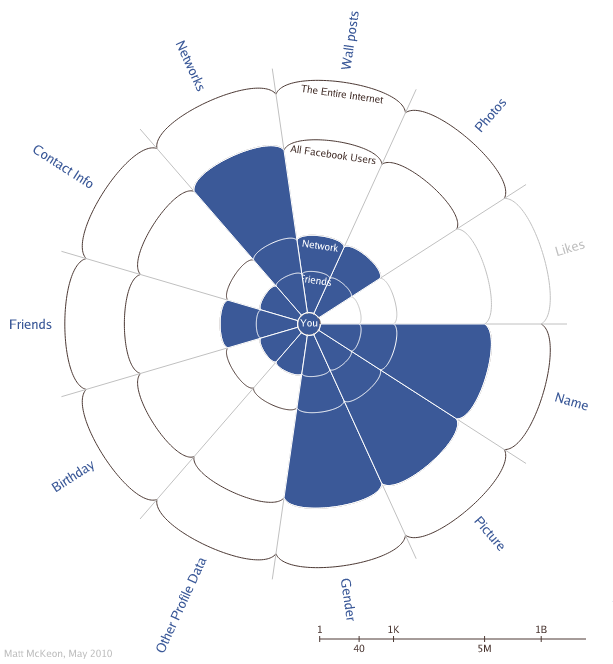
\includegraphics[width=0.80\textwidth, height=100mm]{dp2005.png}\\ 
    \hline
    2006 & In addition to the default privacy settings in 2005, school and specified local area are displayed to all Facebook users.  
    
    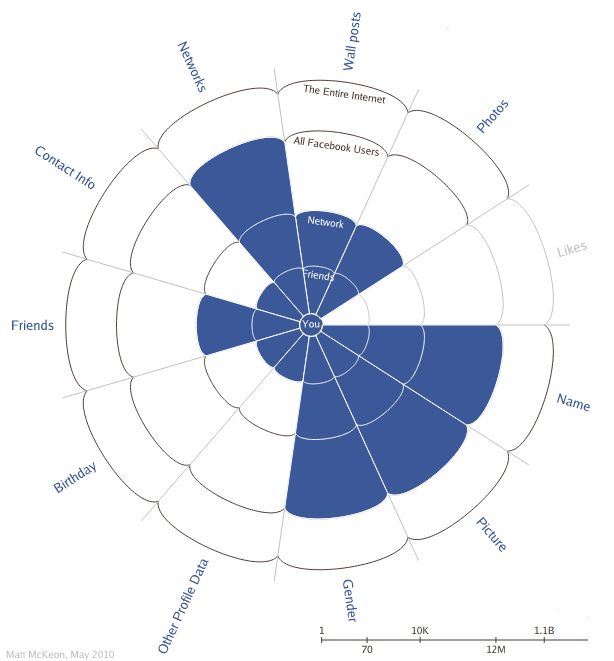
\includegraphics[width=0.80\textwidth, height=100mm]{dp2006.png} \\ 
    \hline
    2007 & Birthday and other profile data became available to the user's specified networks. 
    
    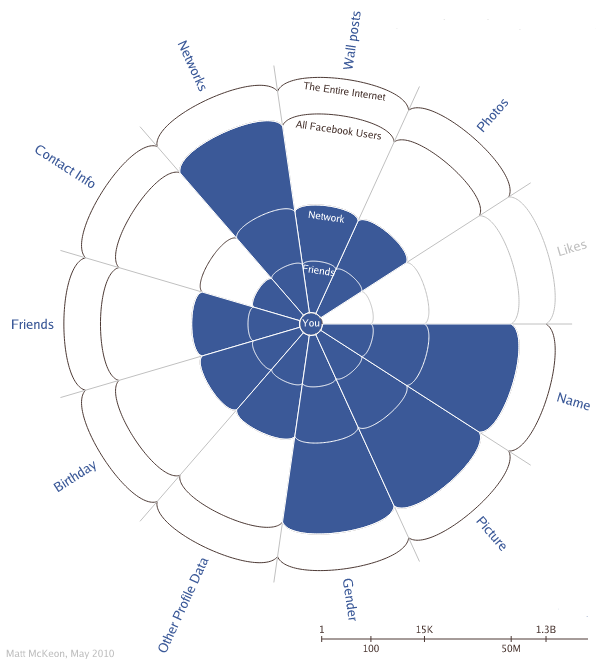
\includegraphics[width=0.80\textwidth, height=100mm]{dp2007.png}\\
    \hline
    November 2009 & Name, profile picture, gender and network became 			available and searchable to the entire Internet. In addition to this, a user's friend-list became visible to all Facebook users. Wall posts, photos, likes, other profile data and birthday became available to friends of friends. 
    
    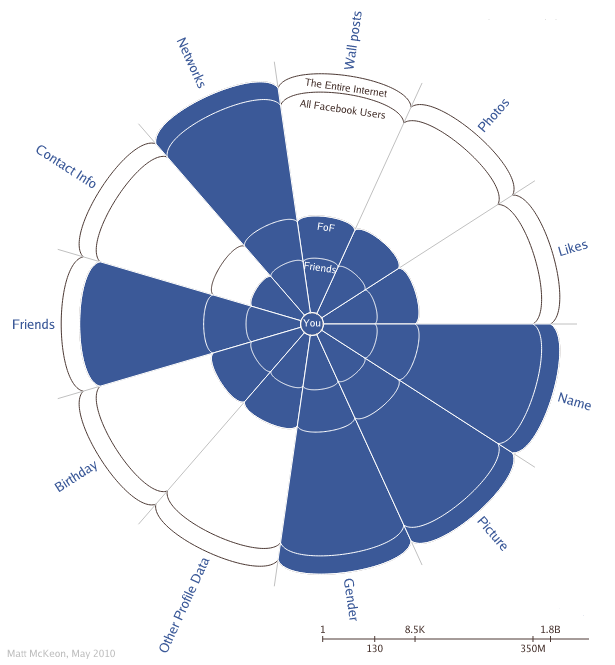
\includegraphics[width=0.80\textwidth, height=100mm]{dp2009nov.png}\\
	\hline
    December 2009 & Likes and a user's list of friends became available to the entire Internet. 
    
    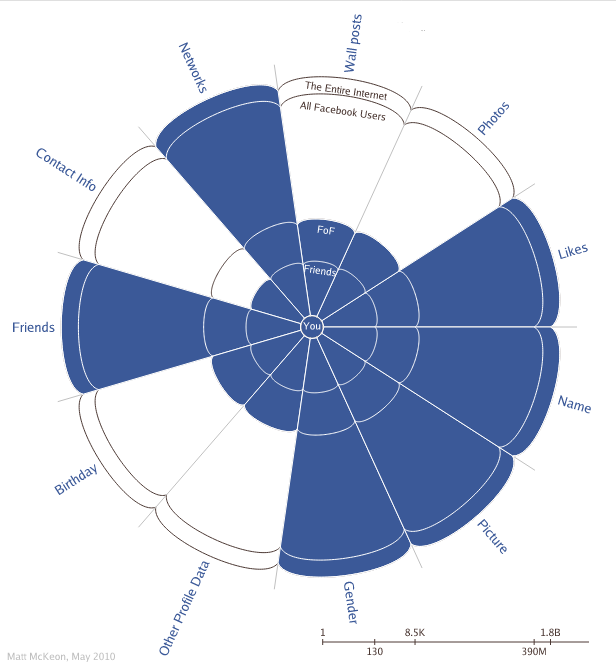
\includegraphics[width=0.80\textwidth, height=100mm]{dp2009des.png}\\
    \hline
    April 2010 & The entire Internet can see everything, except contact info that are limited to friends and birthday which is limited to friends of friends.
    
    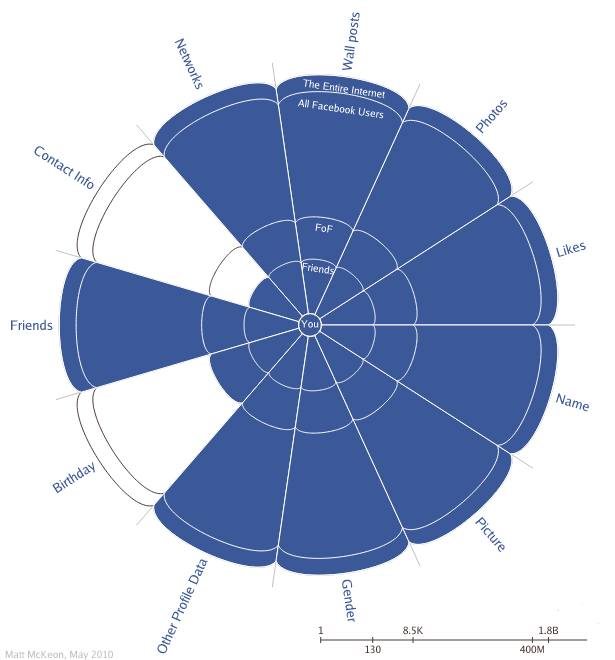
\includegraphics[width=0.80\textwidth, height=100mm]{dp2010april.png} \\
    \hline
    November 2013 & The entire Internet can see everything, except posts you have been tagged in on your Timeline and what is posted by others on your Timeline, which are limited to friends of friends. \\ 
    \hline
   \end{longtable}
\end{center} 


Facebook have had an extreme development. With the consistent growth, the page has gone through a lot of changes, both in appearance and by introducing new features. This encourages, and also in some cases, forces the user to be more public and share more information with others. \tref{tab:dps} displays the development of default settings over the lifetime of Facebook. In 2005, only a user's name, profile picture, gender and network were visible to all Facebook users. Nothing connected to a user's profile was public to all Internet users. This was still in the early days, when Facebook only was available to a limited amount of colleges and high schools.

In 2006 Facebook became publicly available, and everyone with an e-mail address could sign up. It became clear to Facebook that their users did not wish to share all personal information with the entire world. Facebook therefore changed the default settings, and gave the users more options. The users could then decide who they wanted to share information with. A user's name, profile picture, gender, networks, schools and specified local area was available to all Facebook users. Wall posts, photos and the user's list of friends, was limited to networks. Contact information, birthday and other profile data was only visible to a user's friends. 

The only changes that was made from 2006 to 2007, was that birthday and other profile data became visible to a user's networks.

A lot of changes was made to the default privacy settings in November 2009. Name, profile picture, gender and networks, became available to all Internet users. This made it possible to search for a person on, for example, Google and find people's Facebook profiles there. Facebook introduced the feature "like" and the possibility to share with friends of friends, which widely extended the visibility for some content. Wall posts, photos, likes, other profile data and birthday was now visible to friends of friends. All Facebook users could see a person's list of friends, but contact information was still only visible to a user's friends. Just a month later, December 2009, also a user's likes and list of friends became visible to the entire Internet. 

Facebook is becoming more and more public, and the number of users is rapidly growing. In April 2010, everything except contact information, that was limited to friends, and birthday, that was limited to friends of friends, was publicly visible to the entire Internet. Anyone and everyone could now see almost everything connected to a user's Facebook profile. 

In addition to Facebook's introduction of Timeline (see \ref{subsec:timeline} for more information), they also introduced new settings for members under the age of 18. All the settings that were default set to "public" for a regular user, was changed to "friends of friends", and work and school networks for the ones under the age of 18. Everyone could see what others posted on a user's Timeline, as well as posts the user had been tagged in.

Today, in 2013, the entire Internet can see everything, except posts you've been tagged in on your timeline and others posts on your timeline, which are limited to friends of friends. We will take a closer look at how the default privacy settings are today, and explain the changes possible in section \ref{subsec:default2013}. 

Even though Facebook makes the default settings more and more public, it is important to keep in mind that they also let the users change everything and decide themselves who they would like to share information with.   


\subsection{Default Settings 2013}
\label{subsec:default2013}

To examine the default settings on Facebook as they are today (November 2013), we created a new Facebook profile. \fref{fig:security2013} shows how the default security settings look like in November 2013. As we can see from the Figure, secure browsing is enabled by default. This became default in July 2013, but has been an option since 2011 \cite{secureBrowsing}. 

\begin{figure}[b]
\centering
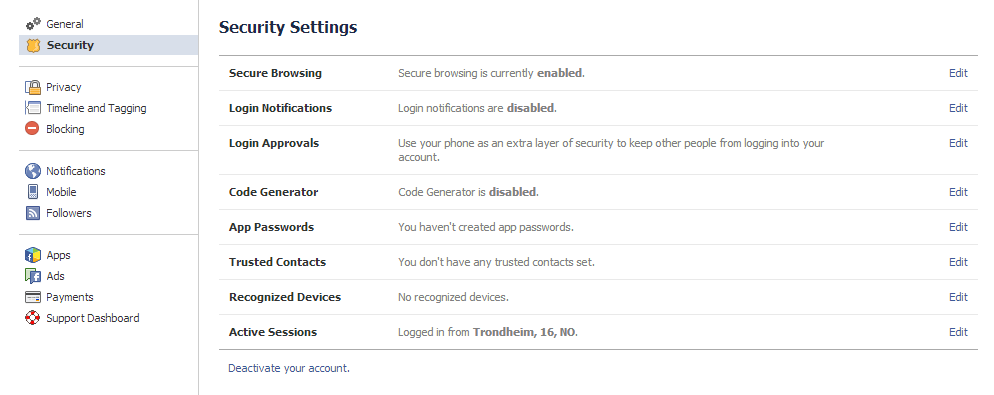
\includegraphics[width=1\textwidth]{default_nov_2013_security.png}
\caption[Default security settings on Facebook November 2013]{\textbf{Default security settings on Facebook November 2013}.} 
\label{fig:security2013}
\end{figure}

\begin{figure}[t]
\centering
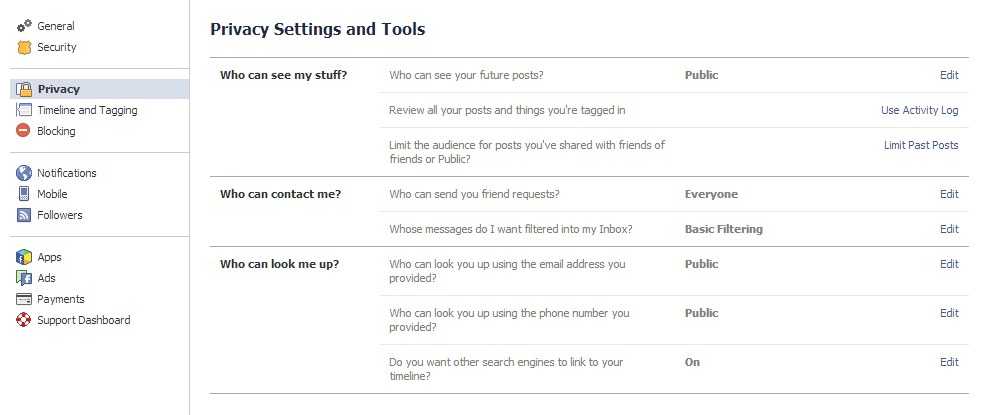
\includegraphics[width=1\textwidth]{default_nov_2013_privacy.png}
\caption[Default privacy settings on Facebook November 2013]{\textbf{Default privacy settings on Facebook November 2013}.} 
\label{fig:privacy2013}
\end{figure}

\begin{figure}[b]
\centering
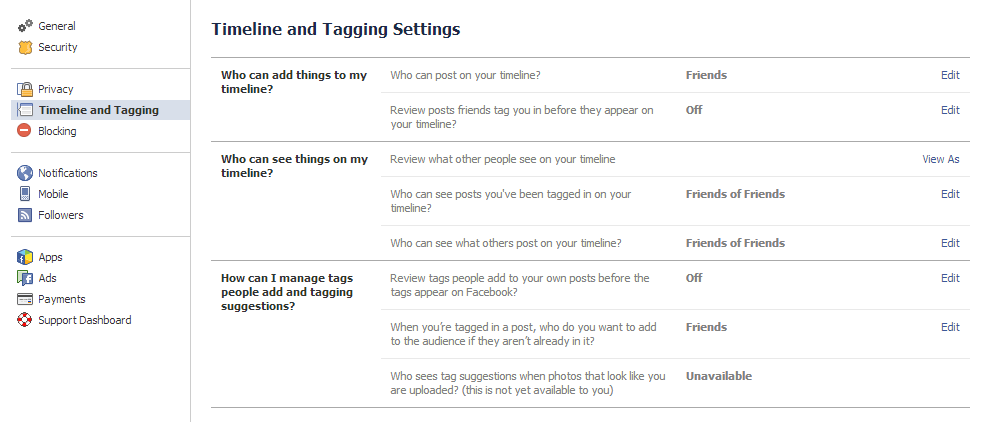
\includegraphics[width=1\textwidth]{default_nov_2013_timelineandtagging.png}
\caption[Default settings for timeline and tagging on Facebook November 2013]{\textbf{Default settings for timeline and tagging on Facebook November 2013}.} 
\label{fig:timelineandtagging2013}
\end{figure}

\begin{figure}[t]
\centering
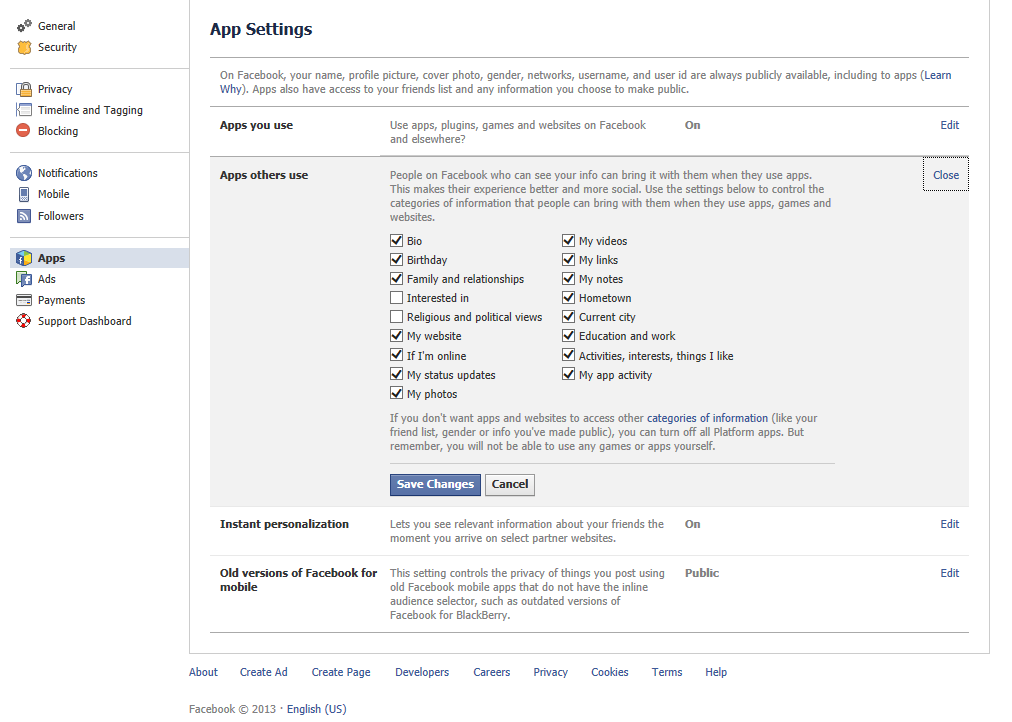
\includegraphics[width=1\textwidth]{default_nov_2013_apps.png}
\caption[Default settings for apps on Facebook November 2013]{\textbf{Default  settings for apps on Facebook November 2013}.} 
\label{fig:apps2013}
\end{figure}

\fref{fig:privacy2013} shows the default privacy settings in November 2013.  \textit{"Who can see your future posts?"} is set to \textit{Public}, which means everyone can view future posts. \textit{"Who can send you friend requests?"} is set to \textit{Everyone}. \textit{"Who can look you up using the email address you provided?"} and \textit{"Who can look you up using the phone number you provided?"} is set to \textit{Public}, which makes it is easier for people to find a user on Facebook if they know the user's email or phone number. The setting \textit{"Do you want other search engines to link to your timeline?"} is turned \textit{on}. This means that, for example, if a user is looked up on Google, the user's Facebook profile will appear in the search. To summarize, the privacy settings are by default \textit{as public as they can be}.

\fref{fig:timelineandtagging2013} shows the default settings for timeline and tagging on Facebook in November 2013. \textit{"Who can post on your timeline?"} is set to \textit{Friends}, which means that only Facebook friends can add things (photos, comments, links, etc.) to the user's timeline. \textit{"Review posts friends tag you in before they appear on your timeline?" }is set to\textit{ off}. This means when a user get tagged in something, it will appear on the user's timeline before the user have had a chance to review it. In most cases this is probably fine, but there may occur a situation where the user do not want the specified content displayed on his/hers timeline. In cases like these it would be desirable to have the review-setting turned on. \textit{"Who can see posts you've been tagged in on your timeline?"} and \textit{"Who can see what others post on your timeline?"} is set to \textit{Friends of friends}. In contrary to those who can post on your timeline, which are friends, friends of friends are able to view the content added to the user's timeline. If you have many friends on Facebook, and these friends have many friends each, the audience are suddenly extremely large. 

\fref{fig:apps2013} shows the default settings for apps on Facebook in November 2013. Usage of apps, plugins, games and websites on Facebook and elsewhere are turned on by default. Under \textit{"Apps others use"}, a user can choose which categories of information that people can bring with them when they use apps, games and websites. As shown in the figure, almost every box is checked of as default. The only exception is "Interested in" and "Religious and political views". Also shown in the figure, instant personalization is enabled by default. The privacy settings for the information you post/have posted using old Facebook mobile apps is set to public as default. 

\subsubsection{Default settings does not preserve privacy} It is safe to conclude that the default privacy settings on Facebook as they are today are far too public. Unless there is made changes to the settings, the timeline will be publicly available, with the exception of posts you've been tagged in and other's posts on your timeline which is "only" visible to friends, and friends of friends. 

\subsection{Default Settings for Teens}

\begin{figure}[t]
\centering
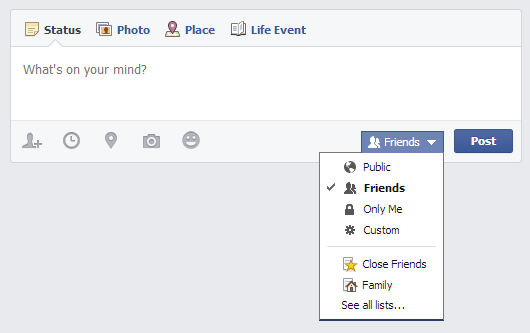
\includegraphics[width=0.8\textwidth]{new_post.png}
\caption[Choosing who can see a status update.]{\textbf{Choosing the audience for a status update.}}
\label{fig:newPost}
\end{figure}

\begin{figure}[b]
\centering
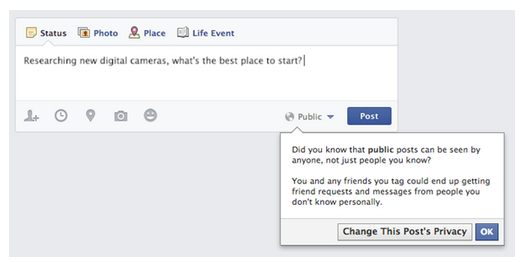
\includegraphics[width=0.8\textwidth]{teensSharePost.png}
\caption[The message shown to teens when posting to the public for the first time]{\textbf{The message shown to teens when posting to the public for the first time.}} 
\label{fig:teensSharePost}
\end{figure}

\begin{figure}[t]
\centering
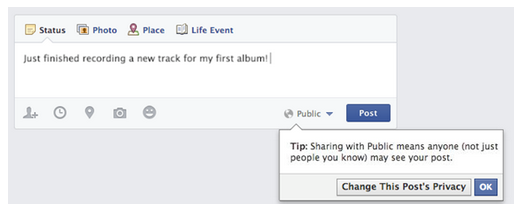
\includegraphics[width=0.8\textwidth]{sharePost.png}
\caption [The message shown to teens when posting to the public, except for the first time]{\textbf{The message shown to teens when posting to the public, except for the first time.}} 
\label{fig:sharePost}
\end{figure}

Each time a user on Facebook share a status update, the user chooses who the post is visible to (see \fref{fig:newPost}). This choice will remain the same for future posts, unless the user decides to change it. Up until today, the default audience is set to "Public", but for teens between 13-17 years, it has been "Friends of friends". On October 16th, 2013, Facebook announced to change the default setting for teens \cite{defaultTeens}. Now the initial audience for posts are "Friends". Teens can now later change this to "Public". This was not an option before. Teens are active users of social networks, and want to be heard, either it is political engagement or an opinion on a movie. Further, Facebook allows teens to turn on Follow, by doing this their public posts will show up in people's news feeds. Facebook designed these changes to improve the Facebook experience for young people. In \cite{defaultTeens} Facebook also makes it clear that they take the safety of teens very seriously, and therefore have created a more extensive warning message, shown in  \fref{fig:teensSharePost}. This message appears when a teen changes the audience for their post. If they continue to post to the public, they will get an additional reminder message, as shown in  \fref{fig:sharePost}.

\section{Facebook Features - Impact on Privacy}\label{sec:facebook_features}

\subsection{News Feed}
\paragraph{}
The News Feed is the first thing shown when logged into a Facebook account. It is a list that constantly is updated. This list includes the activity from friends and info about Pages the user follow on Facebook. Examples of activities that are shown on the News Feed are photos, status updates, links, apps, likes, comments, posts written on timelines and so on. Activities with many comments or likes are often on top of the News Feed. The reason for this is that Facebook uses an algorithm to determine "top stories". This algorithm takes several elements into account when deciding top stories; number of comments, who posted it, and what kind of post it is. The users also have the opportunity to filter their news feed, for example to show only activity from close friends, most recent activities, activities of users in the same network etc. \cite{newsfeed}.

When News Feed was introduced in 2006, many users showed disapproval because they were not given the control over who could see their updates, and were not able to opt out. A consequence of this disapproval was the creation of a group called "Students Against Facebook News Feed", which got 300 000 members in two days. This led to an apology by Zuckerberg: \textit{"We really messed this one up. We didn't build in the proper privacy controls"}. He stated that this was a big mistake on their part \cite{newsfeed2}. 


\subsection{Facebook Platform - Apps}
\label{subsec:app}
The Facebook Platform was launched in May 2007 at a developers conference in San Francisco. This feature enabled a third-party developer to build social applications \cite{BBCFacebookGrowth}. These applications will then be integrated with Facebbok, both mobile and on the web. \textit{"Right now, social networks are closed platforms"}, Zuckerberg said. \textit{"And today, we're going to end that"} \cite{platformStory}. Zuckerberg promised the developers a level playing field, and the opportunity to build apps that could compete with the ones Facebook created. As well as access to the network's, at that time, 24 million users. In \cite{platformStory} McKenzie talk about the launching moment as the moment when Facebook transitioned from having Myspace as a competitor, to getting Google as the competitor. Facebook went from being a wall, and started being a platform. 

18 months after it was launched, Facebook had abandoned the idea of a level playing field, and started baking in features that cut of developers who tried to develop similar products as Facebook. Terms as "Zucked over" became more normal amongst developers. What was once looked at as a beautiful piece of engineering, had become a disappointment. Today the platform is mainly used to distribute games. Zynga, who made the popular game FarmVille, is about the only company who have managed to build their whole business inside the Facebook Platform. The platform did not become what was intended, and as big as everybody was hoping for. According to Facebook's own developers, it has been a hard one to swallow. 

Even though Facebook Platform did not reach out to all the areas originally intended, it is still very popular. By the end of March 2012, there were more than 9 million apps and websites integrated with Facebook through the platform \cite{fbPlatform}.

As mentioned in section \ref{sec:intpriv}, apps is one area that highly concerns the user's interdependent privacy. Facebook Help Center \cite{faceHelp} explain that apps are designed to enhance the user experience with engaging games and useful features. In order for the apps to do this, they ask the user to share personal information. All apps ask for a user's basic information, this consists of name, profile picture, cover photo, gender, networks, user name, and user id. This is information that always is publicly available. Apps also have access to friend-list and any information the user choose to make public. The apps ask for this information to enhance the users experience by personalising content, helping the user find friends that also uses the app, and make sharing of information easier. As well as speeding up the sign-up process, so that the user can start using the game or app right away. 

\paragraph{Application permissions.} As of November 2013, Facebook had 54 permissions divided into 6 different categories \cite{permission}. These categories are email, permissions, extended profile properties, open graph permissions, page permissions and public profile and friend-list. 

\paragraph{Apps privacy control.}In the Facebook settings \cite{facebooksettings} under the tab "Apps" the user can manage apps, see \fref{fig:apps2013}, and control what information that will be shared with apps others use. The user also has the opportunity to turn off all platform applications. The user will then no longer be able to use any games or other applications.

\subsubsection{Installing an Application}
We will now look at the process of installing an application from Facebook App Center. As mentioned earlier, when installing an app, the user will be asked to give permissions to share information. This information vary a lot, some just ask for your basic information, some ask for relationship status, birthday and also permission to post on a user's behalf on the Timeline. We have looked at the very popular application TripAdvisor. According to the site secure.me \cite{secure.me}, TripAdvisor have a poor reputation because it might be a threat to a user's privacy.  

\begin{figure}[t]
\centering
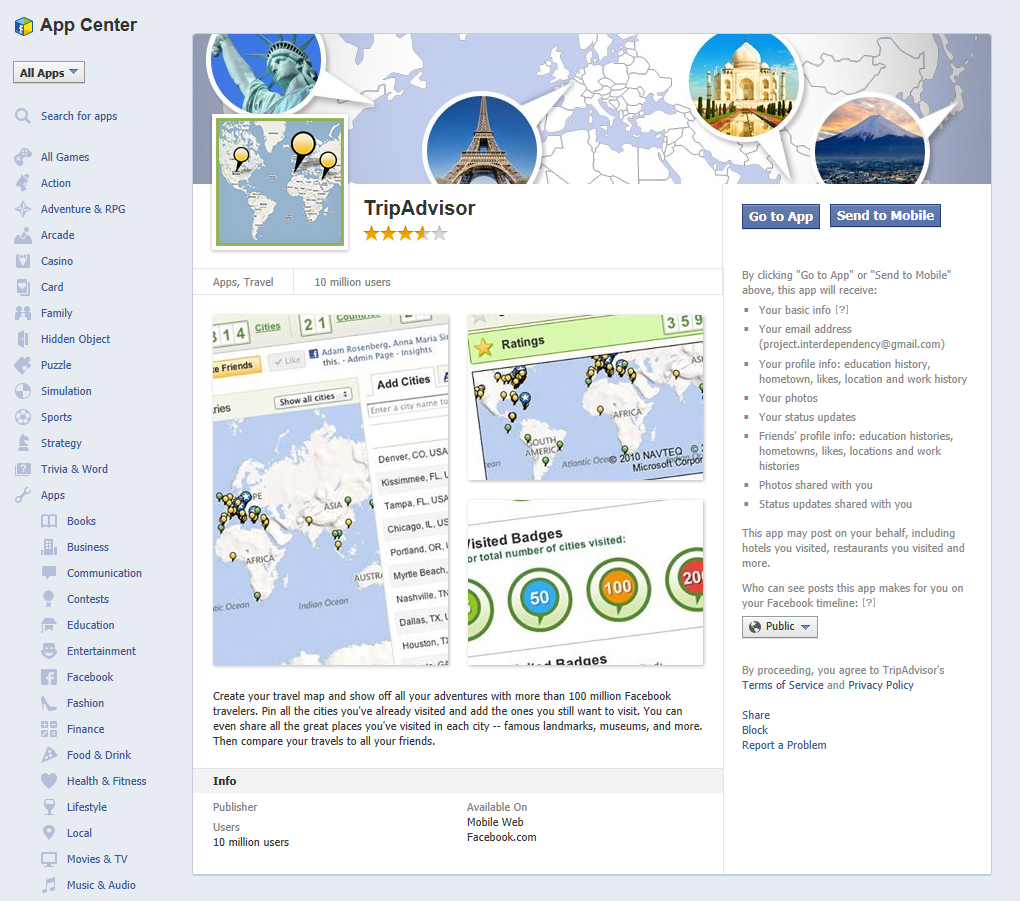
\includegraphics[width=1\textwidth]{tripadvisorpc.png}
\caption[The application TripAdvisor inside Facebook's App Center]{\textbf{The application TripAdvisor inside Facebook's App Center.} } 
\label{fig:tripadvisorpc}
\end{figure}


\paragraph{Installing on a PC.}
When opening TripAdvisor in Facebook's App Center on a personal computer, one gets directed to TripAdvisor's page, as shown in \fref{fig:tripadvisorpc}. The page contains information about the application, as well as the permissions required. These permissions are shown in the top right corner. The permissions that TripAdvisor requires exceeds beyond basic information. We can put these permissions in the following privacy groups; personal privacy, relational privacy and spatial privacy, as mentioned in section \ref{sec:intpriv}. Personal privacy contains the permissions to access personal information about the user like location, education, home town, work history, user's photos, user's status updates, e-mail address and likes. Relational privacy includes retrieving friends' profile information; education history, home town, likes, locations and work history. As well as photos and status updates shared with the user. The last privacy category, spatial privacy, concerns posts that the app post on a user's behalf to the Timeline. By default these posts are set to public, but can easily be changed before installing the app. When pushing the "Go to App"-button, the user automatically give his/hers consent to the required permissions and install the App. This can be misleading, since the user might look for an installation button, or some kind of verification that the installation has started. This may lead to an app being installed without the user knowing. The permissions are all shown, and explained, but not as visible as they used to be before App Center was introduced. \fref{fig:permissions2011} shows the authentication dialogue as of 2011, before App Center was introduced. The user got a pop-up window stating all the permissions requested by the app. The use of pop-up windows like these made it much easier for the user to review the permissions before accepting.


\begin{figure}[t]
\centering
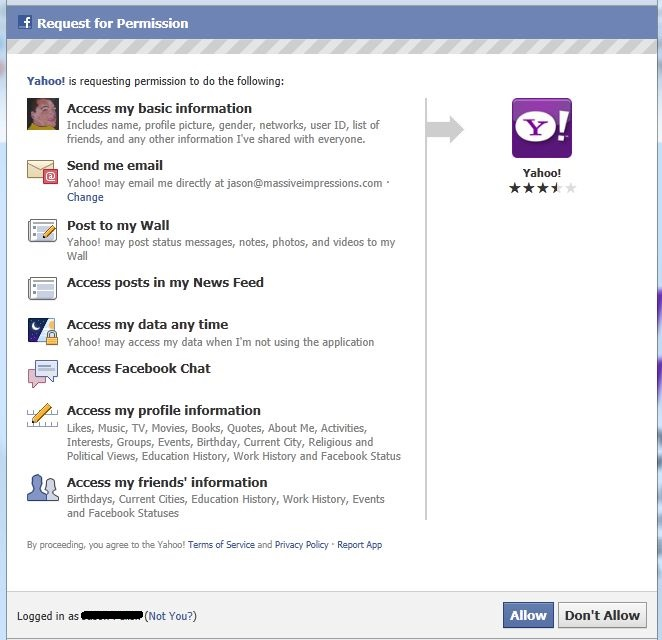
\includegraphics[width=0.8\textwidth]{permissions.jpg}
\caption[Request for permission when installing app anno 2011]{\textbf{Request for permission when installing app anno 2011.} } 
\label{fig:permissions2011}
\end{figure}

\paragraph{Installing on a mobile phone.}
The installation process looks a bit different when installing an app on the Facebook application on a mobile phone. When clicking on the application TripAdvisor in the Facebook mobile app, the user is directed to Apple's App Store or Android's Play Store. \fref{fig:tripa1mobil} shows the application in Android's Play Store. When TripAdviser is installed, the user can choose if he/she would like to connect with Facebook as \fref{fig:tripa2mobil} shows. If the user choose to connect with Facebook the request for permissions will appear in a pop-up window, this is shown in \fref{fig:tripa3mobil}. The user can then choose either to cancel or press OK. When pressing OK, the user gives the app permission to access the requested information stated in the pop-up window. 

\begin{figure}
        \centering
        \begin{subfigure}[t]{0.3\textwidth}
                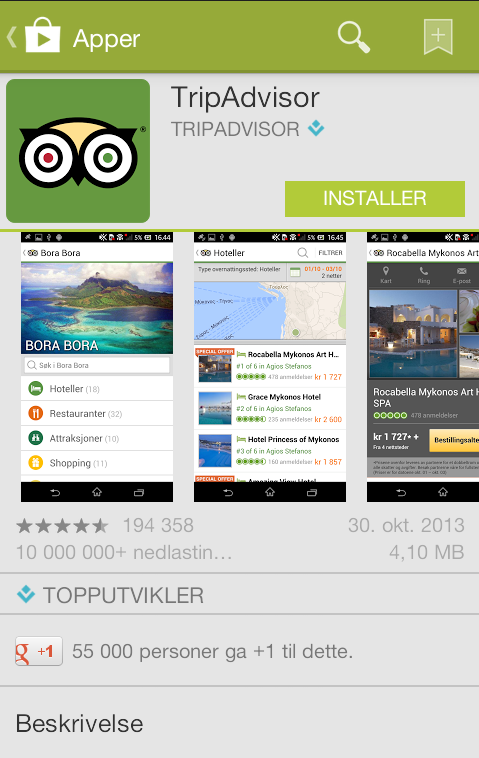
\includegraphics[width=\textwidth]{tripa1mobil.png}
                \caption[Installation page for TripAdvisor]{\textbf{Installation 				page for TripAdvisor.}} 
                \label{fig:tripa1mobil}
        \end{subfigure}%
        ~ %add desired spacing between images, e. g. ~, \quad, \qquad etc.
          %(or a blank line to force the subfigure onto a new line)
        \begin{subfigure}[t]{0.3\textwidth}
                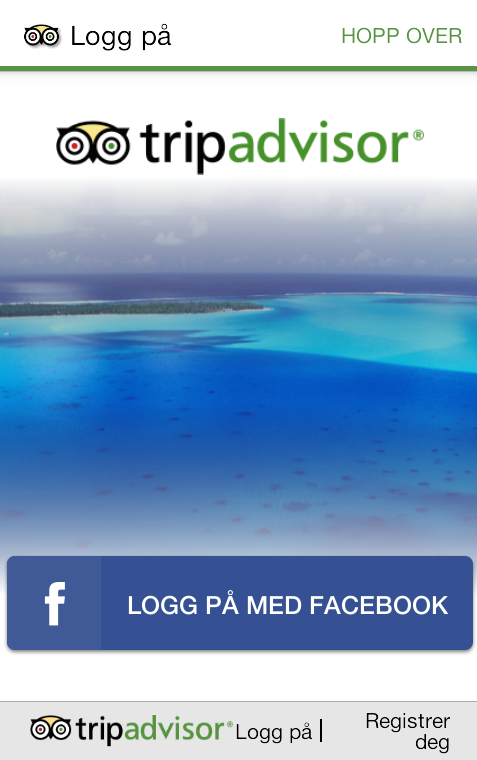
\includegraphics[width=\textwidth]{tripa2mobil.png}
               \caption[The page where you choose "Log in with Facebook"]							{\textbf{The page where you can choose "Log in with Facebook".}} 
                \label{fig:tripa2mobil}
        \end{subfigure}
        ~ %add desired spacing between images, e. g. ~, \quad, \qquad etc.
          %(or a blank line to force the subfigure onto a new line)
        \begin{subfigure}[t]{0.3\textwidth}
                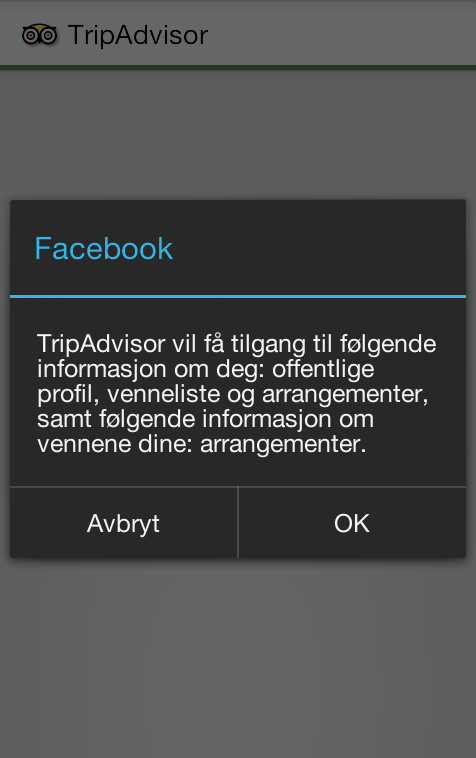
\includegraphics[width=\textwidth]{tripa3mobil.png}
                \caption[Facebook's request for permissions on mobile phone]						{\textbf{Facebook's request for permissions on mobile phone}} 
                \label{fig:tripa3mobil}
        \end{subfigure}
        \caption{Installing TripAdvisor on mobile phone}\label{fig:mobileinstallation}
\end{figure}

%\begin{figure}[t]
%\centering
%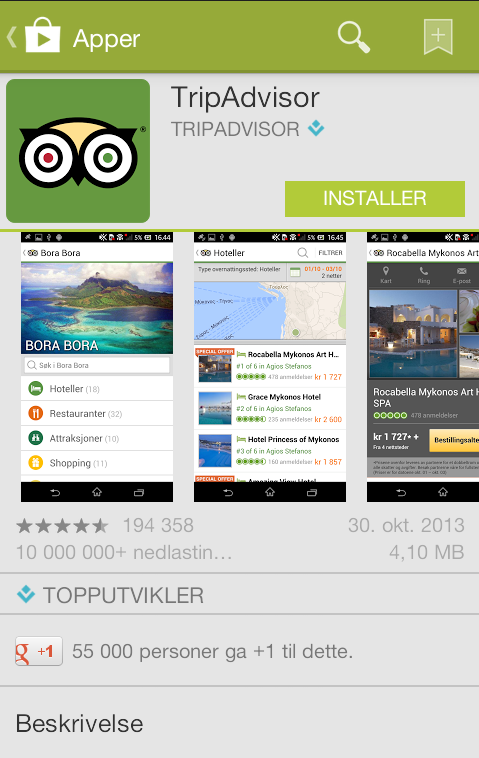
\includegraphics[width=0.5\textwidth]{tripa1mobil.png}
%\caption[Installation page for TripAdvisor]{\textbf{Installation page for TripAdvisor.} This figure shows the installation page for TripAdvisor in Android's Play Store.} 
%\label{fig:tripa1mobil}
%\end{figure}

%\begin{figure}[t]
%\centering
%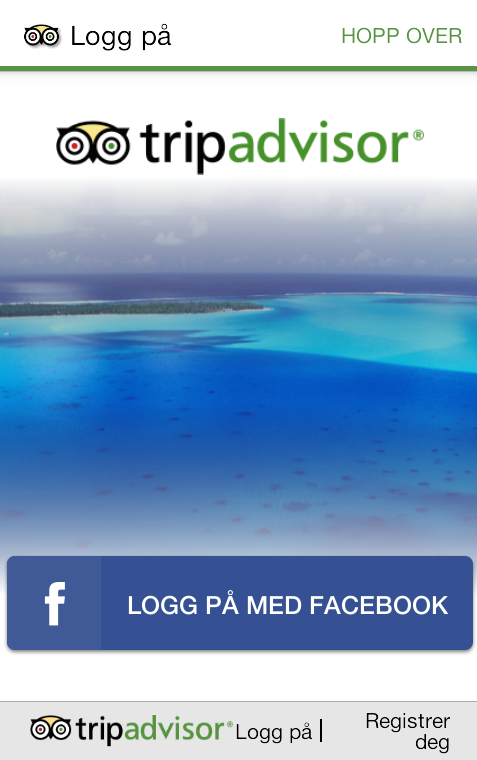
\includegraphics[width=0.5\textwidth]{tripa2mobil.png}
%\caption[The page where you choose "Log in with Facebook"]{\textbf{The page where you can choose "Log in with Facebook".} On this page you can choose whether or not you want to log in with Facebook. If you choose to log in with Facebook you are redirected to the page shown in \fref{fig:tripa3mobil}.} 
%\label{fig:tripa2mobil}
%\end{figure}

%\begin{figure}[b]
%\centering
%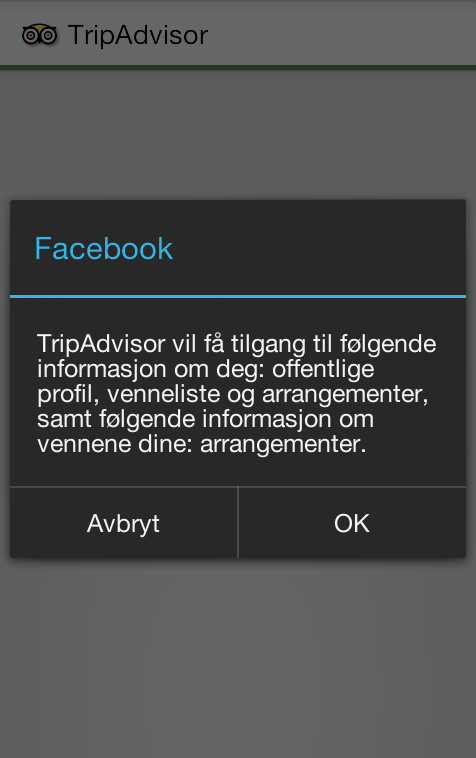
\includegraphics[width=0.5\textwidth]{tripa3mobil.png}
%\caption[Facebook's request for permissions on mobile phone]{\textbf{Facebook's request for permissions on mobile phone} This figure shows the page where Facebook states what permissions they are requesting before you can start using the app. Here you can choose to either cancel or press OK.} 
%\label{fig:tripa3mobil}
%\end{figure}

%Launches app center
%utviklingen utseende
%installere app på web og mobil


\subsection{Beacon}
\paragraph{}
At the end of 2007 Facebook launched the feature Beacon. Beacon was created to help users easily share information from other websites with their Facebook friends \cite{BeaconWebsites}. Beacon was a key part of the Facebook Ads system. The aim was to connect businesses and users, and create more targeted advertising towards the users. 

When Beacon was launched it had 44 partner sites, among these were Live Nation, Fandango, TripAdvisor, STA Travel, eBay, the Knot and Zappos. According to the Facebook announcement \cite{BeaconWebsites} these websites could determine which actions was most relevant and appropriate for a user to share on Facebook. This could be anything from watching a video, a new high score on an online game, posting an item for sale or completing an online purchase. When a user, that is logged on to Facebook, enters a website that is part of Beacon, they will receive a message asking whether they would like to share their actions on Facebook. If a user agree, the user's actions on that page will be shown in their news feed or mini feed, and shared with their friends.  

Beacon received a lot of attention and privacy concerns. Some websites posted to Facebook without first asking the users if they want to share the information. Beacon is a very short piece of code provided by Facebook. The participating websites implement this code on the actions that they would like people to share. An example described in \cite{beaconMarketsPerspective} is with the blog page TypePad. The user have the opportunity to chose whether Beacon should be turned on or not. When creating a post and publishing it the user receives a small pop-up window in the lower right corner stating that you are now sharing this information with Facebook. The pop-up allows the user to decline, but since the window is shown for a limited period of time, the user has to act quickly. When entering Facebook, a message is shown at the top of the user's wall, telling the user that a website have shared information with Facebook. The user then have the opportunity to go through and select whether that website is allowed to share at all, to just friends or to the public.  

Not all websites have created an option for the users to choose for themselves whether or not to opt-in. These websites pushes to Facebook without notifying the users or lets the users select themselves that they want to share it. A much used example of this is a man buying a diamond engagement ring online \cite{ring}. Within hours he starts receiving congratulations from friends and family. The website had posted the purchase on the guys public Facebook page, including a link to the purchase and the price. All his friends received an notification, including his coming fiancée. So much for the surprise engagement.
This is unfortunate for the user, but also for the companies using Beacon, since it puts them in a negative light. Beacon could have been a great asset for companies, and a great way for them to broadcast themselves. 

Another problem was that Beacon only checked that someone was logged into Facebook. When several people use one computer it could create problems, since Beacon was machine specific. One family member, the mother, could be logged in, while her young son was playing an online game, and manages to achieve a new high score. This high score will then be posted on the mother's Facebook news feed. This is not very fortunate for the mother. Beacon only checks that there is a valid Facebook cookie on the machine and then pushes the content to that Facebook user, without any validation. 

In a blog post, Mark Zuckerberg apologized for the way the feature was created and for the handling of complaints in hindsight \cite{Beacon}. Zuckerberg explains that one of the problems with making the system opt-out, was that if a Facebook user forgot to decline something, Beacon still went ahead and posted and shared with the users friends. Further he explains that it took them too long from they started receiving complaints to they were able to decide on a solution to the issues. Facebook released features that gave the users more control, and gave the users the ability to turn off Beacon completely. In addition, Facebook promised their users that they did not save the information Facebook received from the participating websites when the user had chosen to not use Beacon. 

All of Beacon's issues resulted in a lawsuit against Facebook, and some of the participating companies. The lawsuit resulted in a settlement, where Facebook agreed to shut down the feature and gave \$9,5 million to found a new non-profit foundation that would work with online privacy, security and safety \cite{lawsuitB}. Beacon was shut down in September 2009. Beacon is mentioned as one of the darkest marks in the history of social networks.

\subsection{Facebook Connect - "Log in with Facebook"}
From may 2008 users had the ability to connect and log in to other web pages via Facebook, "log in with Facebook". The users are allowed to connect their Facebook identity, friends, and privacy to any website supporting this feature. This was Facebook's first attempt to allow access to user data from Facebook outside of Facebook itself. The important features of Facebook Connect are stated in \tref{tab:connect}.

\begin{center}
\begin{table}[!ht]
\caption{\label{tab:connect}Facebook Connect Features \cite{connect, connect2}.}
    \begin{tabular}{ | l | p{9cm} |}
    \hline
    \textbf{Feature} & \textbf{Description} \\ 
    \hline
    Trusted Authentication & Authentication when users connect their account to a third party. During the user's experience the developer could at any time like to add additional social context. These activities need authentication from the user. In other words, the user have total control over the permissions that are granted. \\ 
    \hline
    Real Identity &  The users can bring information linked to their real identity with them on the web to a third party website. This information includes basic profile information, profile picture, name, friend-list, photos, events, groups etc. \\ 
    \hline
    Friends Access & As mentioned, the users take their friends with them to third party sites. This makes it possible for the developers to add social context to the sites. The user will also get notified if some Facebook friends already have an account on the site.\\
    \hline
    Dynamic Privacy & When the users move around from one place on the web to another, they always bring their privacy settings with them. This is done so one can be sure that their information and privacy settings are updated at any time. In other words, when a user update the privacy settings on Facebook, they will automatically be updated on third party sites.\\
	\hline
    \end{tabular}
   \end{table}
\end{center}


\subsection{Places}
\begin{figure}[t]
\centering
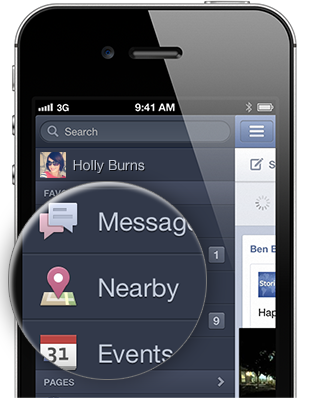
\includegraphics[width=0.3\textwidth]{nearby.png}
\caption[Nearby function on Facebook's mobile application]{\textbf{Nearby function on Facebook's mobile application.}} 
\label{fig:nearby}
\end{figure}

The feature Places was launched in the United States August 2010, and later in the rest of the world. This feature, "Check-in", enables the users to share a place that they really like with their friends, using their mobile device \cite{checkIn}. This can be a café, a new restaurant, a concert or maybe a nice hiking trail. Have you ever been to a concert and found out afterwards that several of your friends also where there? This is what the feature Places solves. You can for example check-in to a concert, and see who else is there, or see which friends are close by. After having checked in at a place, the check-in will appear on your friend's News Feed. It is possible to tag the friends you are with. The user are in control of what is shared and who it is shared with. If a user is tagged in a check-in, they will will always be notified. The default audience is "Friends", unless the users choose to share differently, for example with "Everyone".

\begin{figure}[t]
\centering
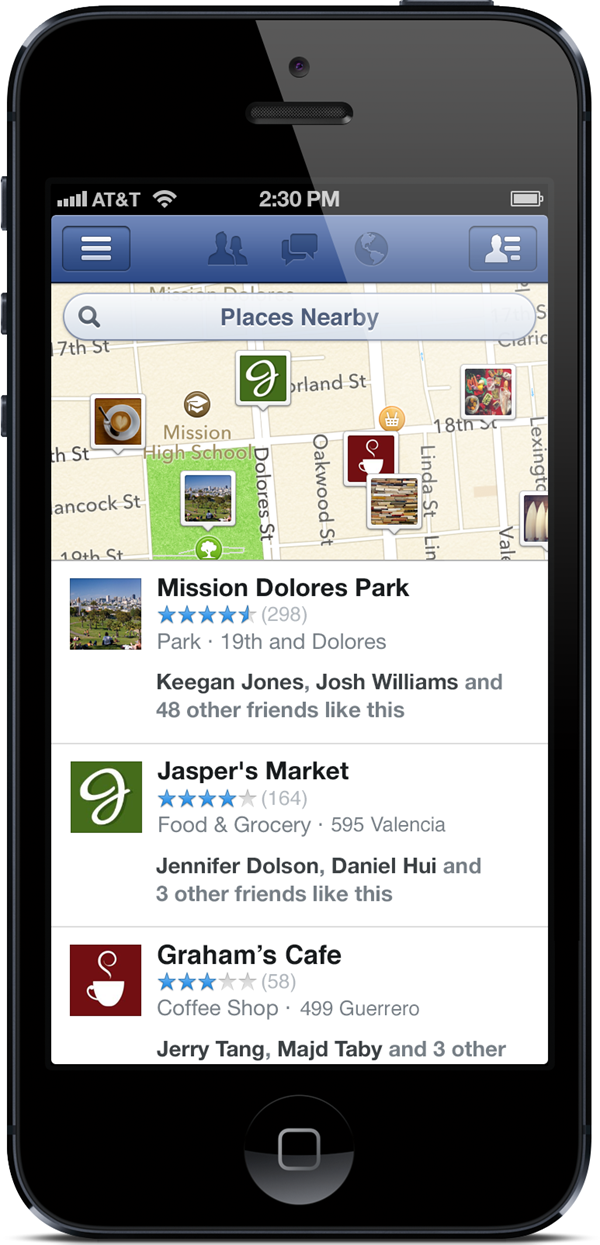
\includegraphics[width=0.3\textwidth]{places.png}
\caption [The "Places nearby" feature]{\textbf{The "Places nearby" feature.} Displaying places close to their current location.} 
\label{fig:places}
\end{figure}

This feature is also used with third-party applications, like TripAdvisor or other travel planning applications. They collect a user's check-ins to generate a map that shows where the in the world the user has been. So if you are planning on going to Paris, you can see who else has been there and also at what places, restaurants etc., they have checked in to. 
When you write a post on Facebook you can decide if you would like to add a location to the post. When creating the post, the user can also decide the audience. On the mobile phone it is a little bit different. Here the location setting is located in the phone settings and not in the Facebook settings. The location service on the phone can get your location by using Wi-Fi, mobile network or GPS signals. When a user writes a post and wants to add a location, the phone asks the user to turn on GPS, this to get a more accurate location. If the users decide not to turn it on, he/she can write in a location, for example "Oslo", and Facebook will suggest places. A feature on the Facebook's mobile application is "Places nearby". Here the user can see what places that are close to their current location, and which friends that have liked the place or/and checked in there, and ratings from other users. This is shown in \fref{fig:nearby} and \fref{fig:places}. A user also have the ability to add locations to photos that they post themselves or that others have posted. 


\subsection{Timeline}
\label{subsec:timeline}
Facebook Timeline was introduced in December 2011 \cite{EvolutionOfFacebook}. This feature made the entire history of the users visible: your posts, posts by others, likes, photos, links, pages liked, comments and other things that the user have shared on Facebook. The timeline showed much more than the old profile, and it was far more visual \cite{timeline}. On the top of a user's timeline it is room for a big photo. This photo is called a \emph{cover photo}. Cover photos are publicly available, and it is not possible to change the settings for them. The user can of course choose which photo is wanted as the cover photo, or just choose to not have a photo there at all. When scrolling down your timeline, you see photos, posts etc. and different events in your life in order of when they happened in time \cite{timeline}. The user can look at it as the story of his/hers life. The user get the opportunity to "go back in time" and fill in the blanks. If the user want to emphasize, for example an event or a photo, the user can highlight it with a star, or on the other hand, hide something from the timeline that is not wanted there. 

\subsubsection{Privacy concerns regarding Facebook timeline}
When Timeline was introduced many people became overwhelmed by the changes, and felt they lost control over their privacy. When a user agreed to start using timeline, the user got a certain period of time to review and edit the timeline before making it public. This gave the users the opportunity to clean up their timeline before everyone else could view the content of it. Cleaning up the timeline can be done using something called the "Activity Log" \cite{activitylog}. The Activity Log is basically a list over everything ever done in connection with a user on Facebook, either done by the user or by others. The activity log also makes it easy to view and change the audience for the different "activities". \fref{fig:activitylog} shows an example of an activity log. On the left side you see types of content. If a user want to view for example "Posts by others", he/she can do so. To the right you see a list of the years and months. A user can click on a year or month, and review the activity from that year/month \cite{activitylog}. If the user are an active user of Facebook, reviewing the whole activity log can be very time consuming. 

\begin{figure}[t]
\centering
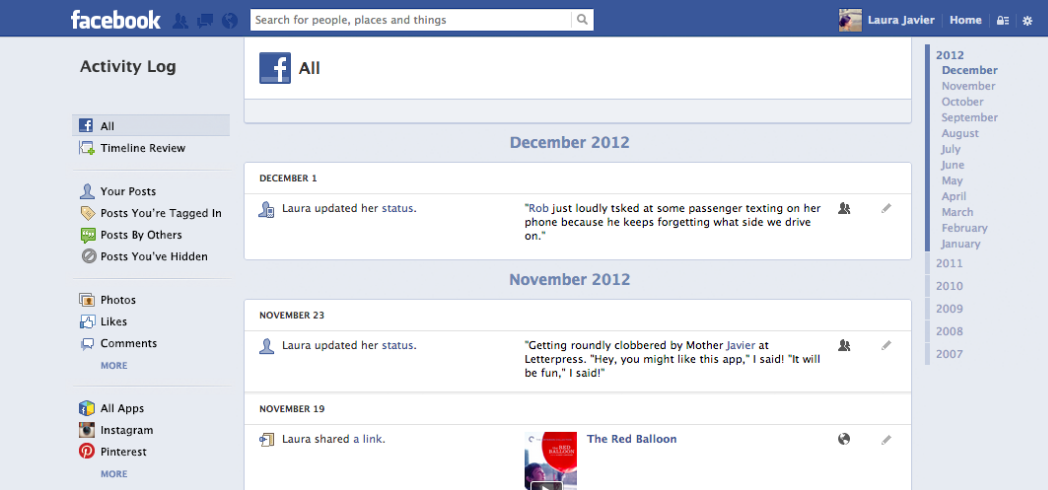
\includegraphics[width=1\textwidth]{activity_log.png}
\caption [Example of an activity log on Facebook.]{\textbf{Example of an activity log on Facebook.}} 
\label{fig:activitylog}
\end{figure}

\paragraph{}
The introduction of Timeline was not in itself a privacy breach since the user had, and still have, the opportunity to decide what he/she want visible on the timeline, and what content should preferably be hidden. On the other hand, there are people who are extra exposed when Facebook introduced new major changes, like the timeline. Let us refer back to section \ref{sec:relatedwork_facebookprivacy} in Chapter \ref{chp:relatedwork}, where we highlighted some of the findings from the survey addressed in \cite{whocares}. Boyd and Hargittai concluded their paper, based on their survey and findings, that experience and Internet skill is important to take into account in regard to how people handle their privacy settings on Facebook. Since familiarity with technology plays a role in how people handle their Facebook privacy/security settings, one might assume that the less skilled people get more exposed when Facebook changes the outline of the default privacy settings. 
This can be seen in the context with the introduction of the timeline. The less skilled users of Facebook that perhaps do not know how to change their privacy settings, probably was left extra exposed when the timeline was introduced. Their timeline may have shown, and may still show, more than they actually would prefer. 

There also exits privacy settings connected to a user's timeline under "Timeline and tagging" in the Facebook settings (see section \ref{sec:privacy_on_facebook}). A user can regulate who can add things to the timeline, and who can see things on the timeline. Under "Privacy" the user can also regulate who can see your future posts. 

\subsection{Graph Search}
Graph Search is a semantic search engine introduced in a beta version by Facebook in March 2013. During the summer 2013 the Graph Search became available for everyone using Facebook with US English language \cite{graphsearchnet}. The old search bar at the top of the page is replaced with a larger search bar, Graph Search \cite{graphsearchfb}. The Graph Search enables the users to search using natural language queries, and not just keywords. In addition to this the search results will be based on both relationships and content \citep{graphsearchnet}. Two examples are "Photos of 'friend's name' are tagged in" and "Restaurants in Oslo, Norway visited by my friends". The basic idea is that the users are given the possibility to search Facebook for different information (photos, people, places etc.) in a specific subset, specifying the queries \cite{graphsearchew}. To emphasize how specific the search can be, we will provide you with an example. Let us say you met someone at a party and the only thing you know about the person is the name, where the person goes to school and you know that the person is a friend of one of your Facebook friends. Then you can write a query which reads as follows: \textit{"People named 'name of the person' that are friends with 'name of the common acquaintance' and who go to 'name of school'"}. Off course this may not give the outcome you wished for, if the person for example have not given any information about where he/she goes to school on Facebook. Just having the opportunity to perform such queries gives the user more power, and makes it easier to connect to new people. 

Zuckerberg says that Graph Search is centred around "making new connections" \cite{graphsearchew}. Facebook emphasizes that the purpose of Graph Search is not to replace traditional web search. The Graph Search concerns, on the other hand, the filtering of all photos and all connections on Facebook. Since Facebook is the largest online social network in the work, it is \textit{not just a few} photos and connections available, but over 240 billion photos and over 1 trillion connections. The choices a user have made in the settings determine what friends and others can see when they conduct a Graph Search \cite{graphsearchtips}. If a photo is set to "Only me" no one else can find it in the search, it it is set to "Friends" friends can find it in their search, and if it is set to "Public" anyone who searches for it can find it. Graph Search is, in other words, a good tool for viewing as many photos as possible of people who are not your Facebook friends. The photos of a user that are public will come up in a Graph Search regardless of how the user have set the privacy settings. As long as someone have posted a photo of a person as public, the entire Facebook can find and view this photo via Graph Search. So if you are interested in viewing pictures of a specific person who is not your friend on Facebook, it is not necessary to start digging through numerous albums and so on, but rather with a quick search. 

A limited group of people got access to Graph Search in January 2013. During a introductory press conference, Mark Zuckerberg stated that Graph Search was in it's early stages, and that it will take years to complete it. He said: \textit{"Graph Search is a really big project, and it's going to take years and years to index the whole map of the graph"}. After the introduction of Graph Search, many questions was brought up regarding the privacy issues. One of the issues brought up, was that the tool makes it easier for people to retrieve information and photos about other people, who do not want this content to be available and seen. The fact is that people only get to view content they already could view, but it makes it much easier to find this content. Facebook  assured that Graph Search does not affect the privacy of minors. They stated that identifying information about those between the ages of 13 and 17 would only be shared with the minor's friends of friends \cite{graphsearchcw}. 

Graph search is for the time being still only available for users using US English language on their Facebook, but is a work in progress. Facebook has stated that further work on the feature deals with searching across posts, comments and mobile \cite{graphsearchcw}. 


\subsection{Facebook Removes Search Privacy Setting}
October 11, 2013, Facebook announced that they will remove the setting that until now had made it possible for Facebook users to hide from the ability to be looked up on the Internet \cite{searchSetting}. The change only affected the users that had not changed the setting: "Do you want other search engines to link to your timeline?" under "Who can look me up?". Facebook explained the removal of the feature by it being outdated, and that there are several other ways to find a person's Timeline. Mark Zuckerberg argued that users should not have information they do not want everyone to see set to public anyway, so it is irrelevant whether or not someone can find you on Google. 
 

\section{Zuckerberg's Thoughts}

\paragraph{}
Zuckerberg once said this about Facebook in a one of his meetings: \textit{"I mean, one way to look at the goal of the site is to increase people’s understanding of the world around them, to increase their information supply"}, he said. \textit{"The way you do that best is by having people share as much information as they are comfortable with. The way you make people comfortable is by giving them control over exactly who can see what"} \cite{MeMedia}.

\paragraph{}
This comment from Zuckerberg brings out his thoughts around the privacy issues. He wants the users of Facebook to be comfortable with sharing information, and give them confidence by giving them control. In general Facebook's privacy settings and restrictions have protected the users. They can easily change the setting and decide who can see what. Zuckerberg firmly means that a user should not post comments or pictures of things one do not want anybody else to see. And if a user does so, the user has to take the blame for it, not Facebook. Zuckerberg was once asked about pictures put on Facebook of students drinking at an East Coast college, which led to some students being expelled. His answer was: \textit{"First of all, it's pretty stupid if you put up pictures of you doing drugs on Facebook. I think that that's just sort of the deviant behavior on the very far end of the distribution. I bet that those kids do not post pictures of them doing drugs on Facebook anymore."} He added that he meant this was a \textit{"pretty shitty way to learn that"} \cite{MeMedia}.

\paragraph{}
Mark Zuckerberg wrote this in a letter to possible investors \cite{LetterToInvestors}: \textit{"Facebook was not originally created to be a company. It was built to accomplish a social mission - to make the world more open and connected.} \textit{People sharing more - even if just with their close friends or families - creates a more open culture and leads to a better understanding of the lives and perspectives of others. We believe that this creates a greater number of stronger relationships between people, and that it helps people get exposed to a greater number of diverse perspectives."} Even though Facebook was not originally created to be a company, they pretty fast ended up as one. The reality is not as picture-perfect as their vision. When people share enormous amounts of personal information, their privacy is bound to be affected. 